\subsection{Background}
\begin{frame}{Research objectives}

\textcolor{blue}{Aim}:
    To identify the effect of the RKB approach on collaborative concept mapping in a practical classroom
    % Does the RKB approach affect co-construction of knowledge with concept maps? 
    %If so, to what extent?


\begin{block}{Sub-research questions}
    \begin{enumerate}
        % \item What is the score of group maps? % descriptive RQs
        % \item What is the score of individual maps?
        \item <1-> Is there a significant different between the learning outcomes as a group
        or as an individual?
        \item <2-> How is the pattern of map changes from individual to group?
        \item <3-> How is the affective response of the students while following the activities?
\end{enumerate}
\end{block}

%% The study focuses on identifying the effectiveness from the end-products 
%% (collaborative maps), the patterns of map changes from individuals to groups, 
%% and the perceptions of the students while following the learning activities. 
\end{frame}

\subsection{Analysis methods}

\begin{frame}{Methods}
    \begin{block}{Sub-research questions}
        \begin{enumerate}
        \item <1-2> Is there a significant different between the learning outcomes as a group
        or as an individual?
        \begin{itemize}
            \item <2> evaluation of individual and group concept map by the teacher 
                  as the domain expert
        \end{itemize}
        
        \item <3-4> How is the pattern of map changes from individual to group?
        \begin{itemize}
            \item <4> a propositional-level similarity analysis
        \end{itemize}
        
        \item <5-6> How is the affective response of the students while following the activities?
        \begin{itemize}
            \item <6>c onduct a survey on learners' experiences during each phase of RKB activities
        \end{itemize}
        \end{enumerate}
    \end{block}
\end{frame}

\begin{frame}[allowframebreaks]{Questionnaire on learner's affective response}
    \begin{itemize}
        \item The survey covered items regarding the perspectives of 
              the students on the task itself (e.g., attractiveness 
              and stimulation scales) and the system used (or non-task; 
              e.g., perspicuity scale). 
        \item The questionnaire scales were adopted from the User Experience
              Questionnaire, an Indonesian version (Laugwitz, Held, \& Schrepp, 2008;
              Santoso, Schrepp, Kartono, Yudha, \& Priyogi, 2016). 
        \item The six open-ended questions were given to uncover the positive and
              negative experiences of the students during the experiment.
    \end{itemize}
    
    \begin{figure}[tb]
        \begin{center}
            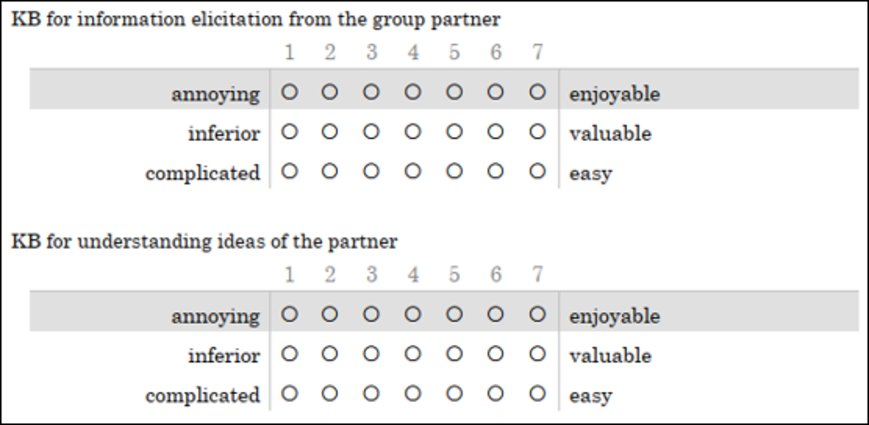
\includegraphics[width=100mm]{images/rqa_questionnaire_closed_items.pdf}
        \end{center}
        \caption{Closed-ended items}
        \label{questionnaire_close}
    \end{figure}
    
    \begin{figure}[tb]
        \begin{center}
            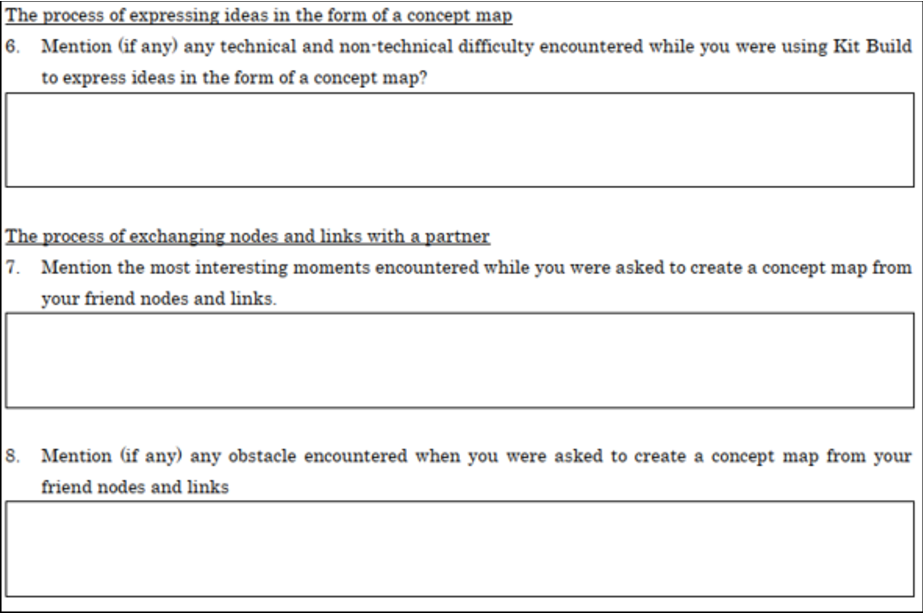
\includegraphics[width=100mm]{images/rqa_questionnaire_open_items.pdf}
        \end{center}
        \caption{Open-ended items}
        \label{questionnaire_open}
    \end{figure}
\end{frame}

\subsection{Results \& discussions}
\begin{frame}{Results (1): Overall group performance}
\begin{table}[tb]
    \caption{Descriptive statistics}
    \label{a1::group_performance}
    \begin{center}
        \begin{tabular}{c|c|c}
            \hline
            & Individual-map score & Group-map score\\
            \hline
            $M$ & 72.21 & 90 \\
            $SD$ & 18.22 & 7.31 \\
            $Min.$ & 41.43 & 75.71 \\
            $Max.$ & 98.57 & 100 \\
            \hline
        \end{tabular}
    \end{center}
\end{table}


\end{frame}

\begin{frame}{Results (1): Scores from the average of individual and group maps, along with the differences between the two scores}

\begin{figure}[tb]
    \begin{center}
        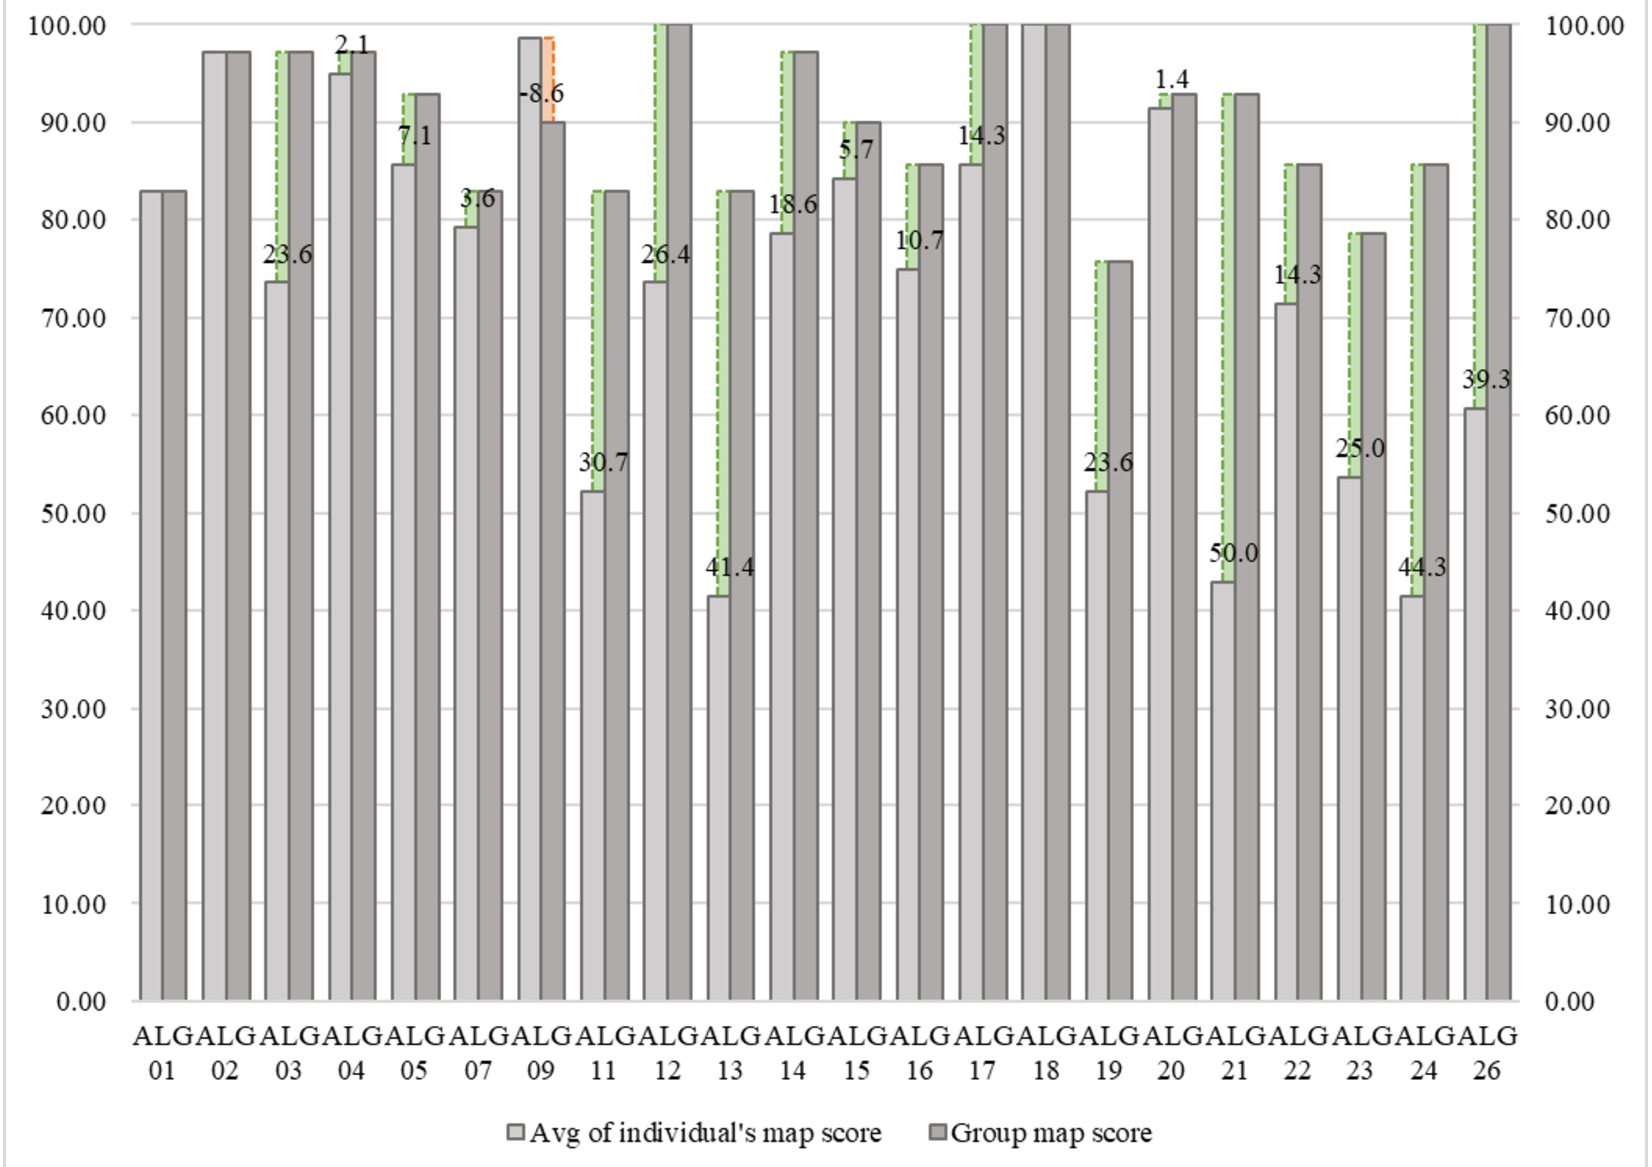
\includegraphics[width=70mm]{images/a1_mapscore_distribution.pdf}
    \end{center}
    %\caption{Scores from the average of individual and group maps, along with the differences between the two scores}
    \label{a1::mapscore_distribution}
\end{figure}

\begin{block}{Finding \#1}
    Almost all groups produce high-quality collaborative products.
\end{block}

\end{frame}

\begin{frame}{Results (1): Distribution of correctness level in all individual and group propositions}
\begin{table}[tb]
    %\caption{Distribution of correctness level in all individual and group propositions}
    \label{dist_correct}
    \begin{center}
        \begin{tabular}{ p{5cm}|p{2cm}|p{2cm}  }
            \hline
            Level of correctness & Individual-map (\%) & Group-map (\%)\\
            \hline
            The true proposition & 64 & 81 \\
            The false proposition with a minor error & 5 & 7 \\
            The false proposition with a moderate error & 10 & 7 \\
            The false proposition with a fatal error & 21 & 5 \\
            \hline
        \end{tabular}
    \end{center}
\end{table}
\end{frame}

\begin{frame}{Results (2): Questionnaire results - closed-ended items}
    \begin{figure}[tb]
    \begin{center}
        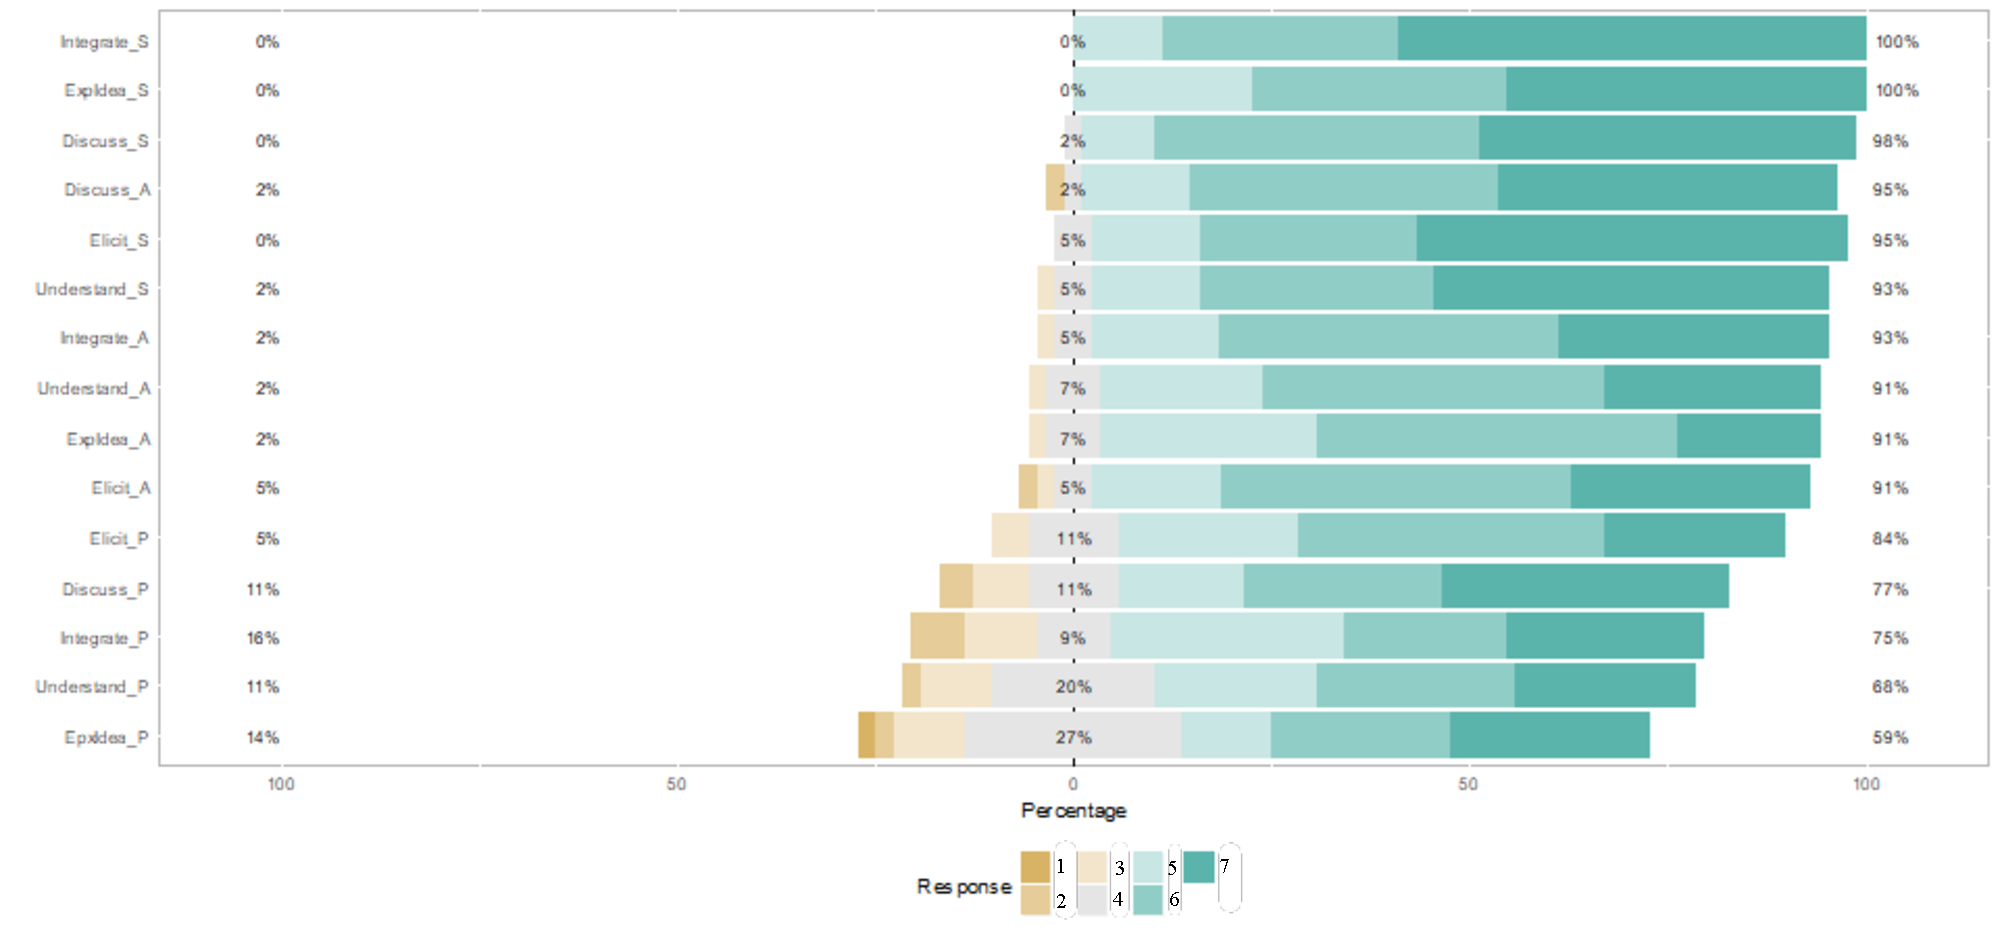
\includegraphics[width=100mm]{images/rqa_affective_response.pdf}
    \end{center}
    %\caption{Sample of individual maps and group map generated by group ALG12}
    \label{a1::questionnaire}
\end{figure}
\end{frame}
\begin{frame}{Results (2): Questionnaire results - open-ended items}
\begin{itemize}
    \item <1> More than half of the students (60\%) agreed that the most attractive phase was the phase when they could \textcolor{teal}{see the difference} between the initial concept map and the reconstructed map (e.g., “I was glad to see the different way to connect the nodes by my friend").
    \item <2> The KB visualization of difference map also helped them to \textcolor{teal}{realize their mistakes} (14.9\%, e.g., “I realized if I have misconceptions or incorrect notions”) and made them \textcolor{teal}{understand  their partner} (8.9\%, e.g., “I need to guess and try to understand perspectives of my friend's concept map.”)
    \item <3> The KB links aided students in \textcolor{teal}{detecting alternatives perspectives} as well (25.5\%, e.g., “It is interesting to see the variety of my friends’ concepts and discussing it together.”)
    \item <4> Students faced \textcolor{purple}{difficulties in integrating different perspectives} (15\%), especially when they had many differences (6.4\%)\item 
\end{itemize}
\end{frame}
\begin{frame}{}
\begin{block}{Finding \#2}
    Students show positive acceptance toward the activities, though they the task was not so easy. 
\end{block}

\end{frame}

\begin{frame}{Results (3): Pattern of map changes}

\begin{figure}[tb]
    \begin{center}
        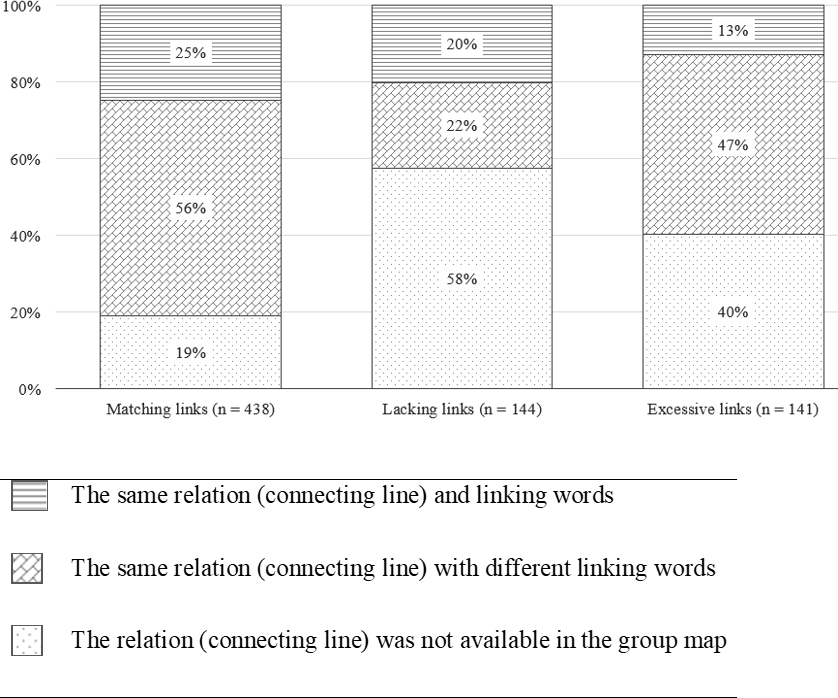
\includegraphics[width=50mm]{images/dist_match_links.pdf}
    \end{center}
    \caption{Proportions of the individual propositions taken from the system,with  the  matching,  lacking,  and  excessive  links,  compared  to  the  group propositions}
    \label{a1::map_sample_1}
\end{figure}

\end{frame}
\begin{frame}{Results (3): Pattern of map changes based on the visualization}

    \begin{columns}
        \begin{column}{0.5\textwidth}
            \begin{center}
                \begin{figure}[tb]
                    \includegraphics[width=55mm]{/images/rqa_map_patterns_b.pdf}
                    %\caption{Scatter plot of group prior knowledge similarity and normalized gain from individual to collaborative map}
                    %\label{prior_gain}
                \end{figure}
            \end{center}
        \end{column}
        \begin{column}{0.5\textwidth}  %%<--- here
            \begin{center}
                \begin{figure}[tb]
                    \includegraphics[width=50mm]{/images/rqa_map_patterns_a.pdf}
                    %\caption{Scatter plot of group comprehension level and normalized gain from 
                    %individual to collaborative map}
                    %\label{comprehension_gain}
                \end{figure}
            \end{center}
        \end{column}
    \end{columns} 
    
    
    %\begin{figure}[tb]
    %\begin{center}
    %    \includegraphics[width=50mm]{images/rqa_map_patterns_a.pdf}
    %\end{center}
    
    %\label{a1::map_sample_1}
    %\end{figure}
\end{frame}


\begin{frame}{Results (3): Pattern of map changes based on the visualization}
%    \begin{figure}[tb]
%    \begin{center}
%        \includegraphics[width=80mm]{images/rqa_map_patterns_b.pdf}
%    \end{center}
%    \caption{The  number  of  propositions  from  the  individual  to  the  groupmaps were categorized by the link types in the KB-map, the similarity be-tween the KB-map proposition and the group-map proposition, and the levelof group proposition correctness}
%    \label{a1::map_sample_2}
%\end{figure}
\begin{block}{Finding \#3}
\begin{itemize}
    \item <+->Students \textcolor{teal}{thought deeply} about the propositions and found out the correct representation. 
    \item <+-> Besides, Pearson’s correlation analysis depicted that there was a \textcolor{teal}{moderate positive correlation} between the score differences and the number of excessive links presented in the KB analyzer (R(21) = 0.58, p < .01).
\end{itemize}
\end{block}

\end{frame}
